\begin{table*}[!t]
\centering
\small
\setlength{\tabcolsep}{3.5pt}
\caption{\textbf{Benchmark positioning and property comparison.}}
\vspace{-2mm}
\renewcommand{\arraystretch}{1.10}

\begin{adjustbox}{max width=\textwidth}
\begin{tabular}{@{}
L{1.4cm}
L{2.3cm}
L{8.5cm}
*{5}{M{0.65cm}}
@{}}
\toprule
\textbf{Category} & \textbf{Benchmark} & \textbf{Brief description} &
\textbf{Sci} &
\textbf{Comp} &
\textbf{Inter} &
\textbf{Turn} &
\textbf{Traj} \\
\midrule

\multirow[t]{3}{*}{\textbf{General}} &
\textbf{MMLU} &
Broad subject exam-style evaluation (mostly one-shot). &
\pmark & \xmark & \xmark & \xmark & \xmark \\

&
\textbf{BIG-bench} &
Large heterogeneous task suite for capability probing. &
\pmark & \xmark & \xmark & \xmark & \xmark \\

&
\textbf{HELM} &
Holistic evaluation across scenarios and metrics. &
\pmark & \xmark & \xmark & \pmark & \xmark \\
\addlinespace[1pt]

\textbf{CompGen} &
\textbf{CFQ} &
Compositional generalization benchmark (semantic parsing). &
\xmark & \xmark & \xmark & \pmark & \xmark \\
\addlinespace[1pt]

\textbf{Long ctx} &
\textbf{LongBench} &
Benchmarking long-context understanding and retrieval. &
\xmark & \xmark & \xmark & \pmark & \xmark \\
\addlinespace[1pt]

\textbf{Robust} &
\textbf{Dynabench} &
Dynamic benchmark construction for robustness evaluation. &
\xmark & \xmark & \xmark & \pmark & \xmark \\
\addlinespace[1pt]

\multirow[t]{4}{*}{\textbf{Sci QA}} &
\textbf{ScienceQA} &
Multimodal science QA benchmark (static instances). &
\cmark & \pmark & \xmark & \xmark & \xmark \\

&
\textbf{GPQA} &
Expert-level scientific QA (primarily one-shot). &
\cmark & \xmark & \xmark & \xmark & \xmark \\

&
\textbf{SciBench} &
Static domain expertise probing (isolated fields). &
\cmark & \xmark & \xmark & \xmark & \xmark \\

&
\textbf{MRMR} &
Multidisciplinary multimodal retrieval (23 domains). &
\cmark & \pmark & \xmark & \xmark & \xmark \\
\midrule

\textbf{Diagnostic} &
\textbf{\textsc{XDomainBench}}&
Interactive interdisciplinary reasoning with knowledge composition. &
\cmark & \cmark & \cmark & \cmark & \cmark \\

\bottomrule
\end{tabular}
\end{adjustbox}
\begin{flushleft}
\scriptsize
\textbf{Notes:} 
\textbf{Sci}: designed for scientific/AI4S reasoning;
\textbf{Comp}: supports cross-domain composition \emph{within an instance/session};
\textbf{Inter}: session-level interactive evaluation;
\textbf{Turn}: turn-level diagnostic annotations;
\textbf{Traj}: trajectory-level diagnostic annotations across turns.
$\triangle$ indicates partial/limited support.
\end{flushleft}
\label{tab:benchmark_positioning}
\vspace{-1mm}
\end{table*}

\begin{table}[!t]
\centering
\small
\setlength{\tabcolsep}{3pt}
\caption{\textbf{Comparison of SciQA benchmarks on dataset scale and composition.}}
\vspace{-2mm}
\renewcommand{\arraystretch}{1.0}
\begin{tabular}{@{}L{2.0cm}*{5}{M{0.95cm}}@{}}
\toprule
\textbf{Benchmark} & \textbf{\#Dom} & \textbf{\#Comb} & \textbf{\#Theme} & \textbf{Samples} & \textbf{\#Type} \\
\midrule
\textbf{ScienceQA} & 3 & - & 21 & 10.2 & 1 \\
\textbf{GPQA} & 3 & - & - & 0.4 & 1 \\
\textbf{SciBench} & 3 & - & 9 & 0.7 & 1\\
\textbf{MRMR} & 23 & - & 6 & 1.4 & 1\\
\midrule
\textbf{\textsc{Ours}} & \textbf{20} & \textbf{62} & \textbf{15} & \textbf{8.6} & \textbf{4} \\
\bottomrule
\end{tabular}
\begin{flushleft}
\scriptsize
\textbf{Notes:}
\textbf{\#Dom}: number of domains;
\textbf{\#Comb}: number of domain combinations;
\textbf{\#Theme}: number of interdisciplinary themes;
\textbf{Samples (K)}: sample size in thousands;
\textbf{\#Type}: number of question types.
Empty cells indicate not applicable.
\end{flushleft}
\label{tab:sciqa_comparison}
\vspace{-1mm}
\end{table}

\vspace{-2pt}
\section{Related Work}
\label{sec:related_work}

% \textbf{LLMs for AI4S and interdisciplinary scientific reasoning.}
% LLMs are increasingly adopted in AI4S as a general-purpose interface for scientific knowledge synthesis, integrative reasoning, and workflow support.
% Recent surveys highlight both opportunities and structural bottlenecks, notably the scarcity of high-quality cross-domain data and the challenges of conducting reliable large-scale evaluations~\citep{zhang-etal-2024-comprehensive-survey,zheng-etal-2025-automation}.
% Representative efforts span scientific language modeling~\citep{taylor2022galactica} and broader AI4S breakthroughs that highlight the value of integrating heterogeneous evidence and constraints~\citep{jumper2021highly}.
% However, \emph{interdisciplinary reasoning} in AI4S often requires reconciling coupled constraints and paradigm differences \emph{within a single problem-solving process}, which is a requirement that remains largely unformalized as an explicitly controllable evaluation dimension in existing benchmarks.

\subsection{Interdisciplinary Benchmarking}
\label{sec:related_benchmarking}  

As summarized in Table~\ref{tab:benchmark_positioning}, existing benchmarks generally fall into two categories, yet both capture the compositional nature of interdisciplinary scientific workflows.
The first category includes \textbf{General Evaluations}: MMLU~\citep{hendrycks2021mmlu}, BIG-bench~\citep{srivastava2022beyond}, HELM~\citep{liang2022helm} and \textbf{Specialized Benchmarks}: CFQ~\citep{keysers2020measuring}, LongBench~\citep{bai-etal-2024-longbench}, Dynabench~\citep{kiela-etal-2021-dynabench}, which typically treat each query as an isolated one-shot instance and not explicit control over \emph{how domains are composed} within a single reasoning process.
These circumstances are particularly problematic for AI4S, where \emph{interdisciplinary reasoning} often requires reconciling coupled constraints and paradigm differences \emph{within a single problem-solving process}, which remains largely unformalized as an explicitly controllable evaluation dimension.
The second category focuses on \textbf{scientific Reasoning Benchmarks}, as presented in Table.\ref{tab:sciqa_comparison}: ScienceQA~\citep{lu2022learn}, GPQA~\citep{rein2024gpqa}, and SciBench~\citep{wang2024scibench} advance scientific competence by probing deep knowledge in isolated fields (``silos''), but they focus primarily on evaluating static instances and do not test the dynamic integration required in real research.
Recent work on multidisciplinary benchmarks, such as MRMR~\citep{zhang2025mrmr}, addresses cross-domain challenges in multimodal retrieval across 23 domains, yet focuses on retrieval tasks rather than interactive reasoning, and does not provide trajectory-level diagnostic annotations to understand failure mechanisms.
Moreover, existing benchmarks do not characterize how performance degrades as cross-domain compositions become higher-order, making it difficult to diagnose whether failures stem from missing domain knowledge or limitations in joint reasoning.


\subsection{Interdisciplinary Knowledge Composition}
\label{sec:related_composition}

Cross-domain interdisciplinary reasoning can be viewed as \emph{compositional generalization}, where models must recombine learned knowledge under novel compositions rather than merely recall isolated facts~\citep{lake2018generalization,keysers2020measuring}.
In our setting, \emph{knowledge composition} refers to composing \emph{domain theories and constraints} under a controlled mixture, rather than simply covering multiple subjects.
This perspective motivates treating interdisciplinary reasoning as a high-dimensional \emph{composition space} whose complexity can be scaled and measured via composition order and mixture structure.
However, this formalization remains absent in existing AI4S-oriented evaluations.
  
\subsection{Interactive Reasoning and Diagnostic Evaluation}
\label{sec:related_interactive}

\begin{figure*}[!t]
    \centering
    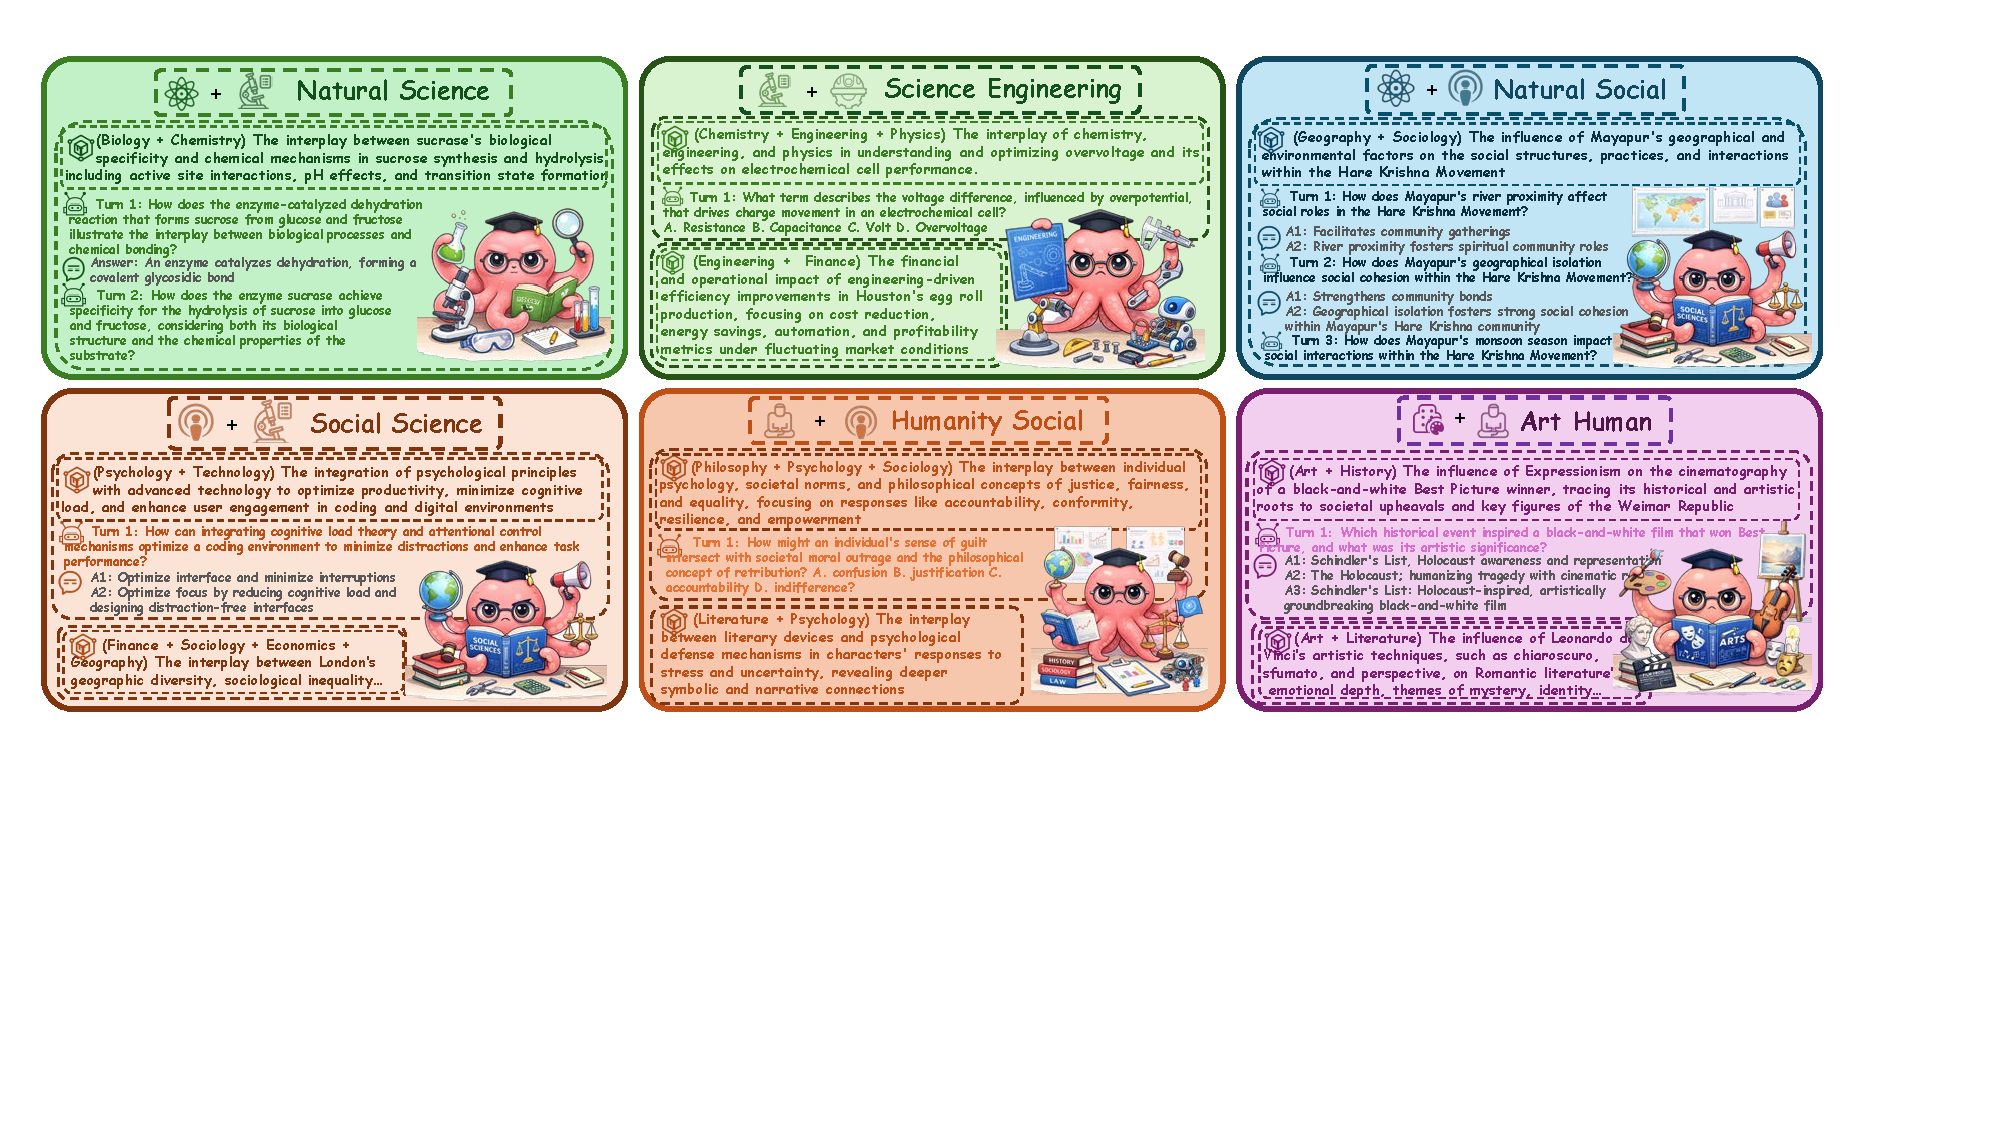
\includegraphics[width=0.99\linewidth]{figures/example.pdf}
    \vspace{-1mm}
    \caption{\textbf{Scientific categories overview of \textsc{XDomainBench}} covering 6 major interdisciplinary categories, 62 combinations.}
    \vspace{-1mm}
    \label{fig:example}
\end{figure*}

\begin{figure}[!t]
    \centering
    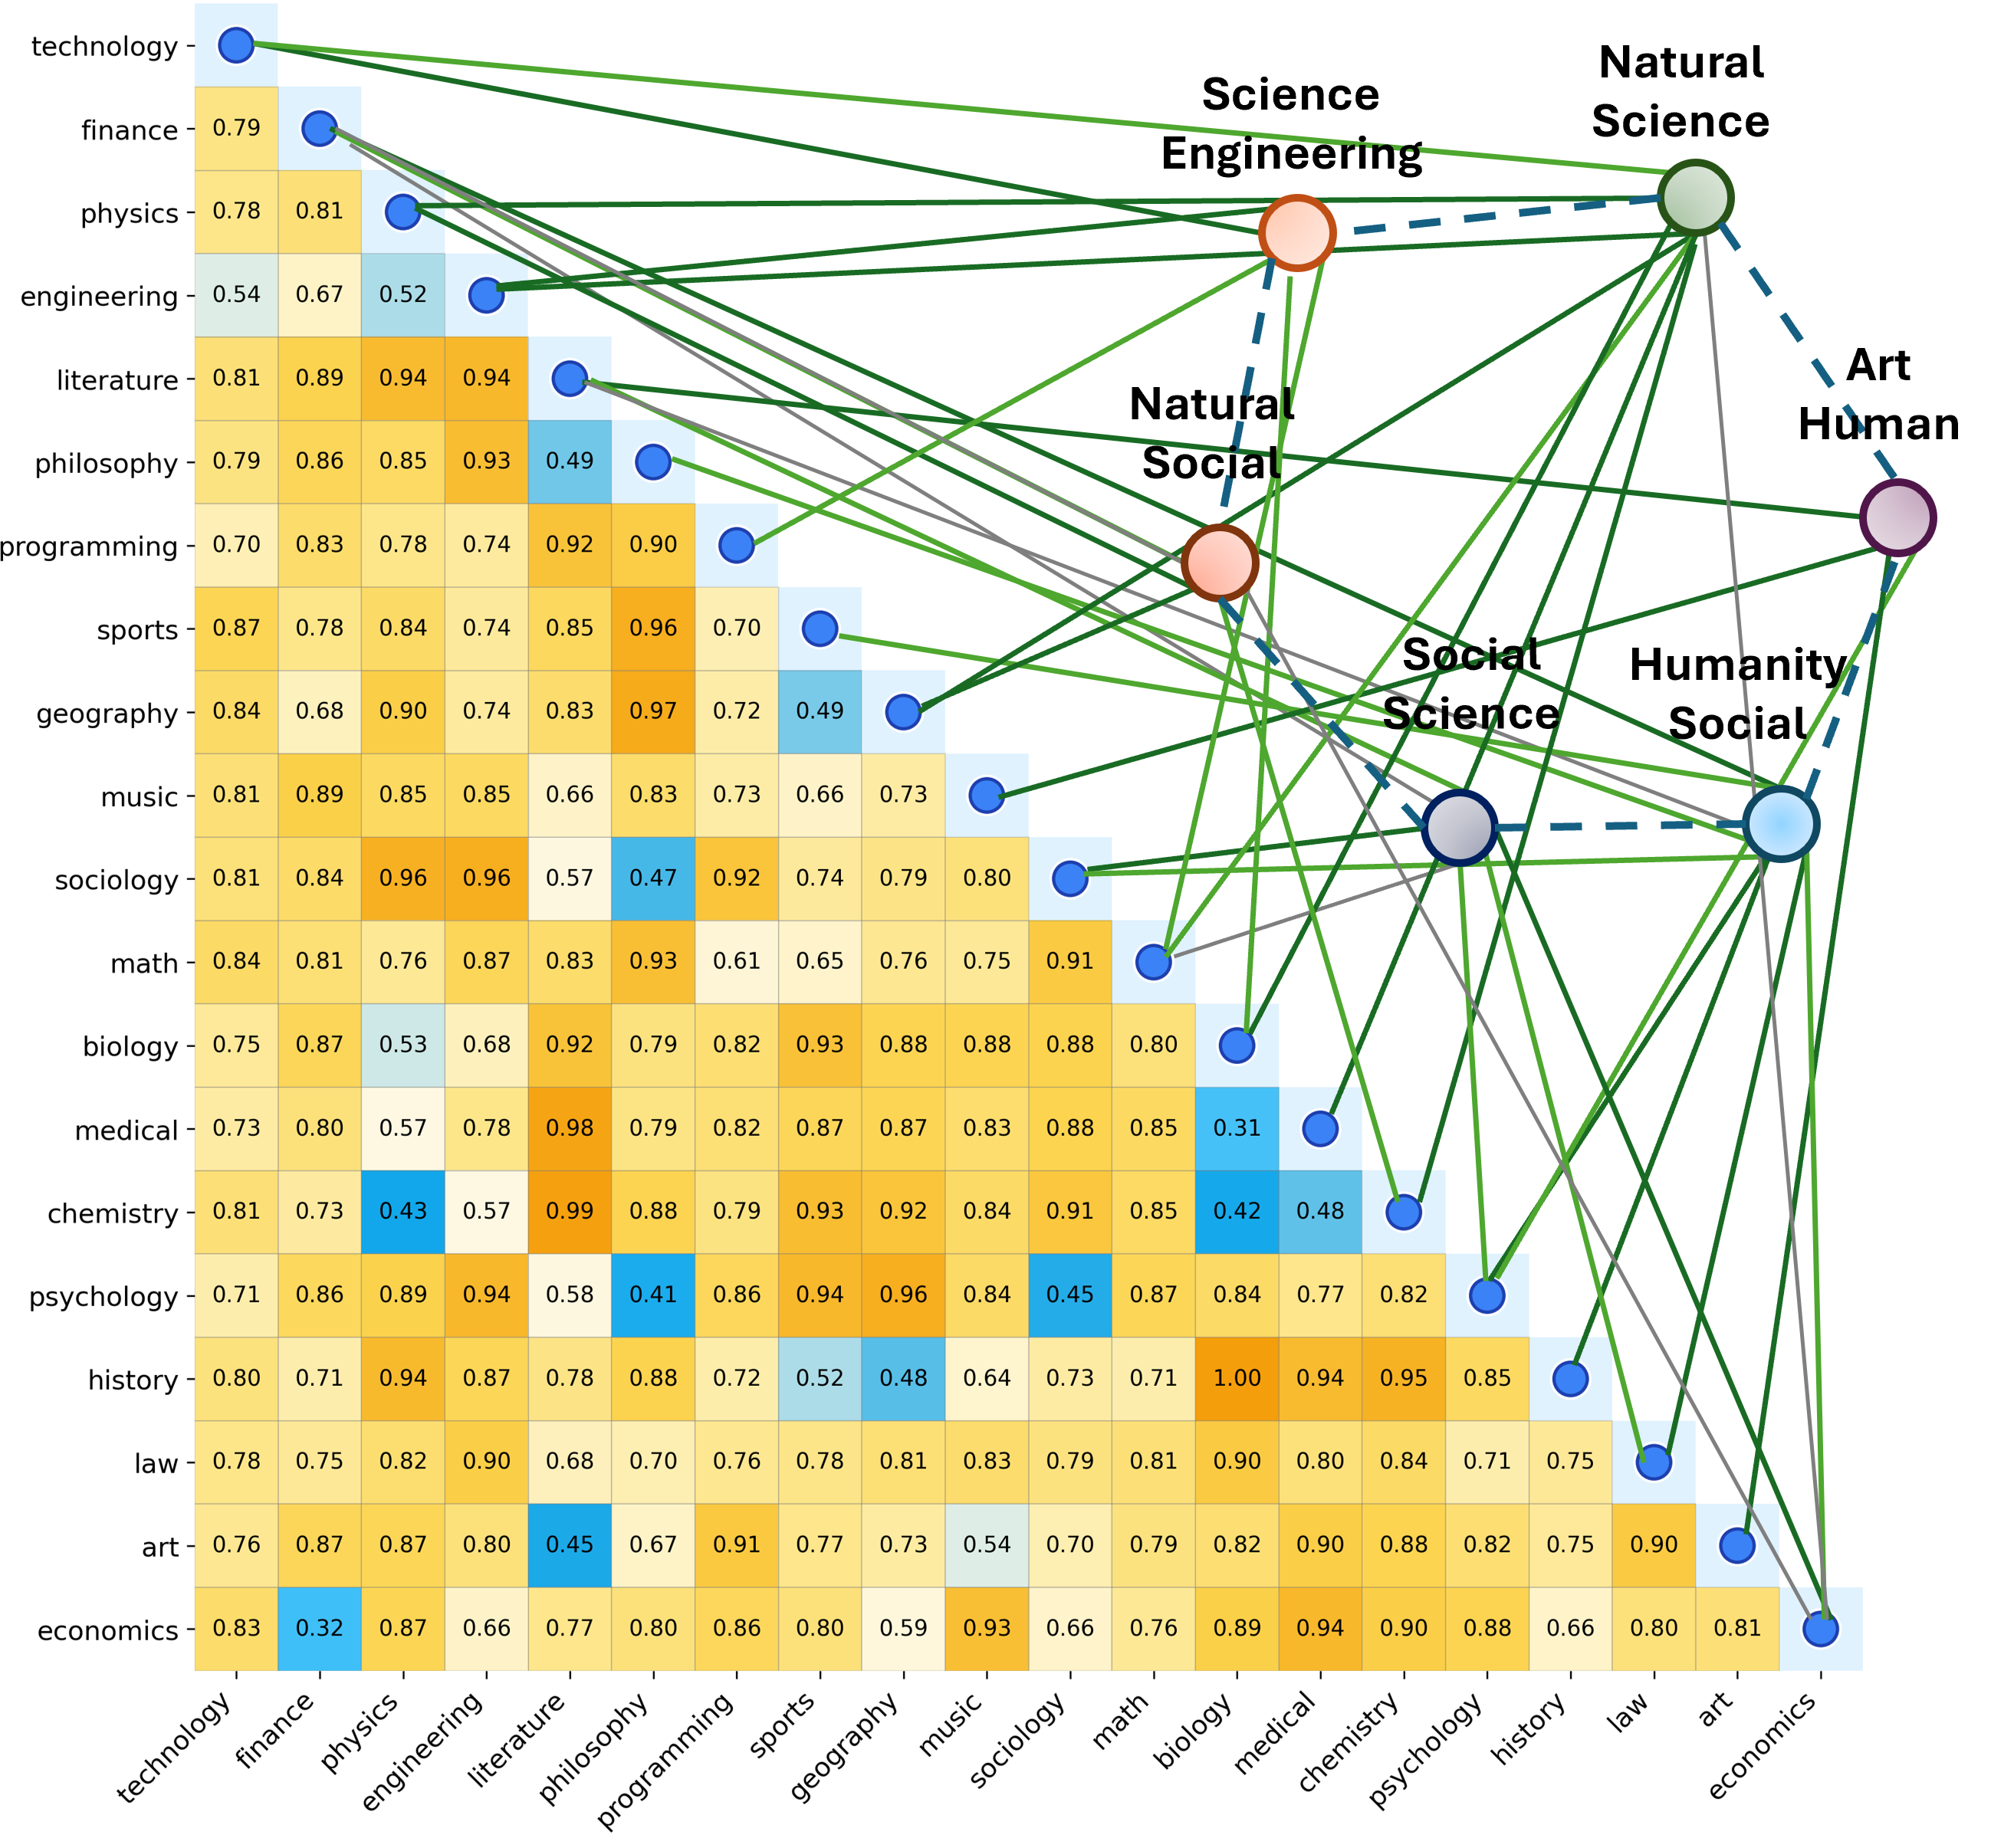
\includegraphics[width=0.99\linewidth]{figures/domain_heatmap.png}
    \vspace{-1mm}
    \caption{\textbf{Inter-domain semantic similarity matrix with domain taxonomy}
     shows cosine similarities between 20 domains, while the network graph categorizes domains into 6 major categories.}
    \label{fig:domain_heatmap}
\end{figure}

Scientific workflows are inherently interactive: questions are refined, intermediate results are reused, and reasoning must adapt as new evidence and constraints appear.
Long-context evaluations, such as LongBench~\citep{bai-etal-2024-longbench}, demonstrate that performance can degrade when crucial evidence is embedded in lengthy contexts~\citep{bai-etal-2024-longbench,liu-etal-2024-lost}.
However, existing benchmarks typically do not provide trajectory-level diagnostic signals (e.g., difficulty fluctuations and domain-mixture shifts) to diagnose \emph{how} and \emph{why} models fail under realistic AI4S workflows.
Robustness-oriented evaluation frameworks~\citep{kiela-etal-2021-dynabench,ribeiro-etal-2020-beyond} highlight that average-case performance scores can obscure systematic failures, yet they lack the composition-space view needed for diagnosing the collapse of interdisciplinary reasoning.
  
% \textbf{Positioning of \textsc{XDomainBench}.}
% In contrast to prior work, \textsc{XDomainBench} targets \emph{interactive interdisciplinary scientific reasoning} by formalizing a high-dimensional \emph{knowledge-composition space} and systematically scaling (i) cross-domain composition order and (ii) mixture structure.
% This design enables controlled measurement of both performance and efficiency degradation, together with mechanism-oriented diagnosis of how interactive session dynamics contribute to error accumulation, reasoning breaks, and domain confusion.

%Table~\ref{tab:benchmark_positioning} summarizes the positioning of \textsc{XDomainBench} relative to representative benchmarks.